\documentclass[]{beamer}
\usetheme{default}

\begin{document}

\frame{\frametitle{}
  \huge
  Introductin of Nasu town
}
\normalsize


\begin{frame}{Summary}
  \begin{figure}[gaiyo]
    \begin{center}
    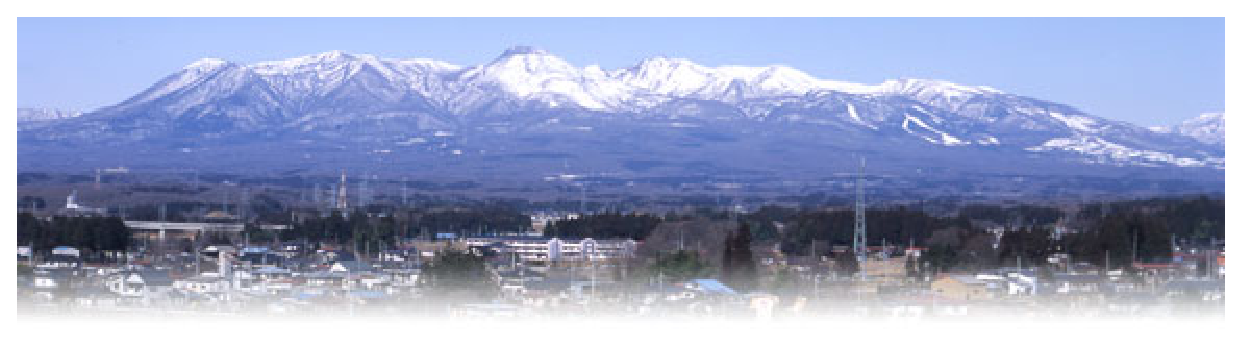
\includegraphics[scale=0.5]{%
      ./pictures/gaiyo.eps}
    \end{center}
  \end{figure}
  
  \begin{itemize}
  \item 栃木県の最北端に位置。\\
  \item 1380年の歴史を持つ温泉があり、日光国立公園「那須温泉郷」として観光の名所となっている。\\
  \item 山麓地帯には、別荘地やテーマーパークがある。\\
  \item 高原地帯には、傾斜地を利用した酪農が続き、中央・東部地区には、水田地帯が広がっている.\\
  \item 南東部の伊王野・芦野地区には源義経、俳人松尾芭蕉に至るまで多くの史跡がある。\\
  \end{itemize}
  
\end{frame}
\begin{frame}{Acces}
  \begin{itemize}
  \item 東京から新幹線で1時間。会津若松から電車で2時間30分ほどである。\\
  \item 日帰りには最適な立地である。\\
  \end{itemize}
   \begin{figure}[map]
    \begin{center}
    \includegraphics[scale=0.5]{%
      ./pictures/bg_train.jpeg}
    \end{center}
  \end{figure}
\end{frame}

\begin{frame}{We'er No.1}
  \begin{itemize}
  \item 那須町は酪農が盛んで、牛乳の生産量は北海道に次いで2位である。\\
    \begin{itemize}
    \item http://grading.jpn.org/y0719010.html\\
    \end{itemize}
  \end{itemize}
  
\end{frame}
\begin{frame}{引用}
  引用元:http://www.town.nasu.lg.jp/index.htm\\
\end{frame}

\end{document}
